\documentclass[a4paper, 10pt]{article}
\usepackage{graphicx}
\usepackage{float}
\usepackage{geometry}
\usepackage[font=small, skip=0pt]{caption}
\usepackage{subcaption}
\usepackage{siunitx}
\usepackage{fancyhdr}
\geometry{margin=20mm}
\setlength{\textfloatsep}{4pt plus 1.0pt minus 2.0pt}
\setlength{\intextsep}{6.0pt plus 1.0pt minus 1.0pt}
\setlength{\belowcaptionskip}{-6pt}

\pagestyle{fancy}
\lhead{COMS30127 Rat Hippocampal Data}

\begin{document}

\section*{COMS30127 Lab M: Analysis of Hippocampal Data}

\subsection*{Neuron Firing Positions}
\begin{figure}[H]
  \centering
  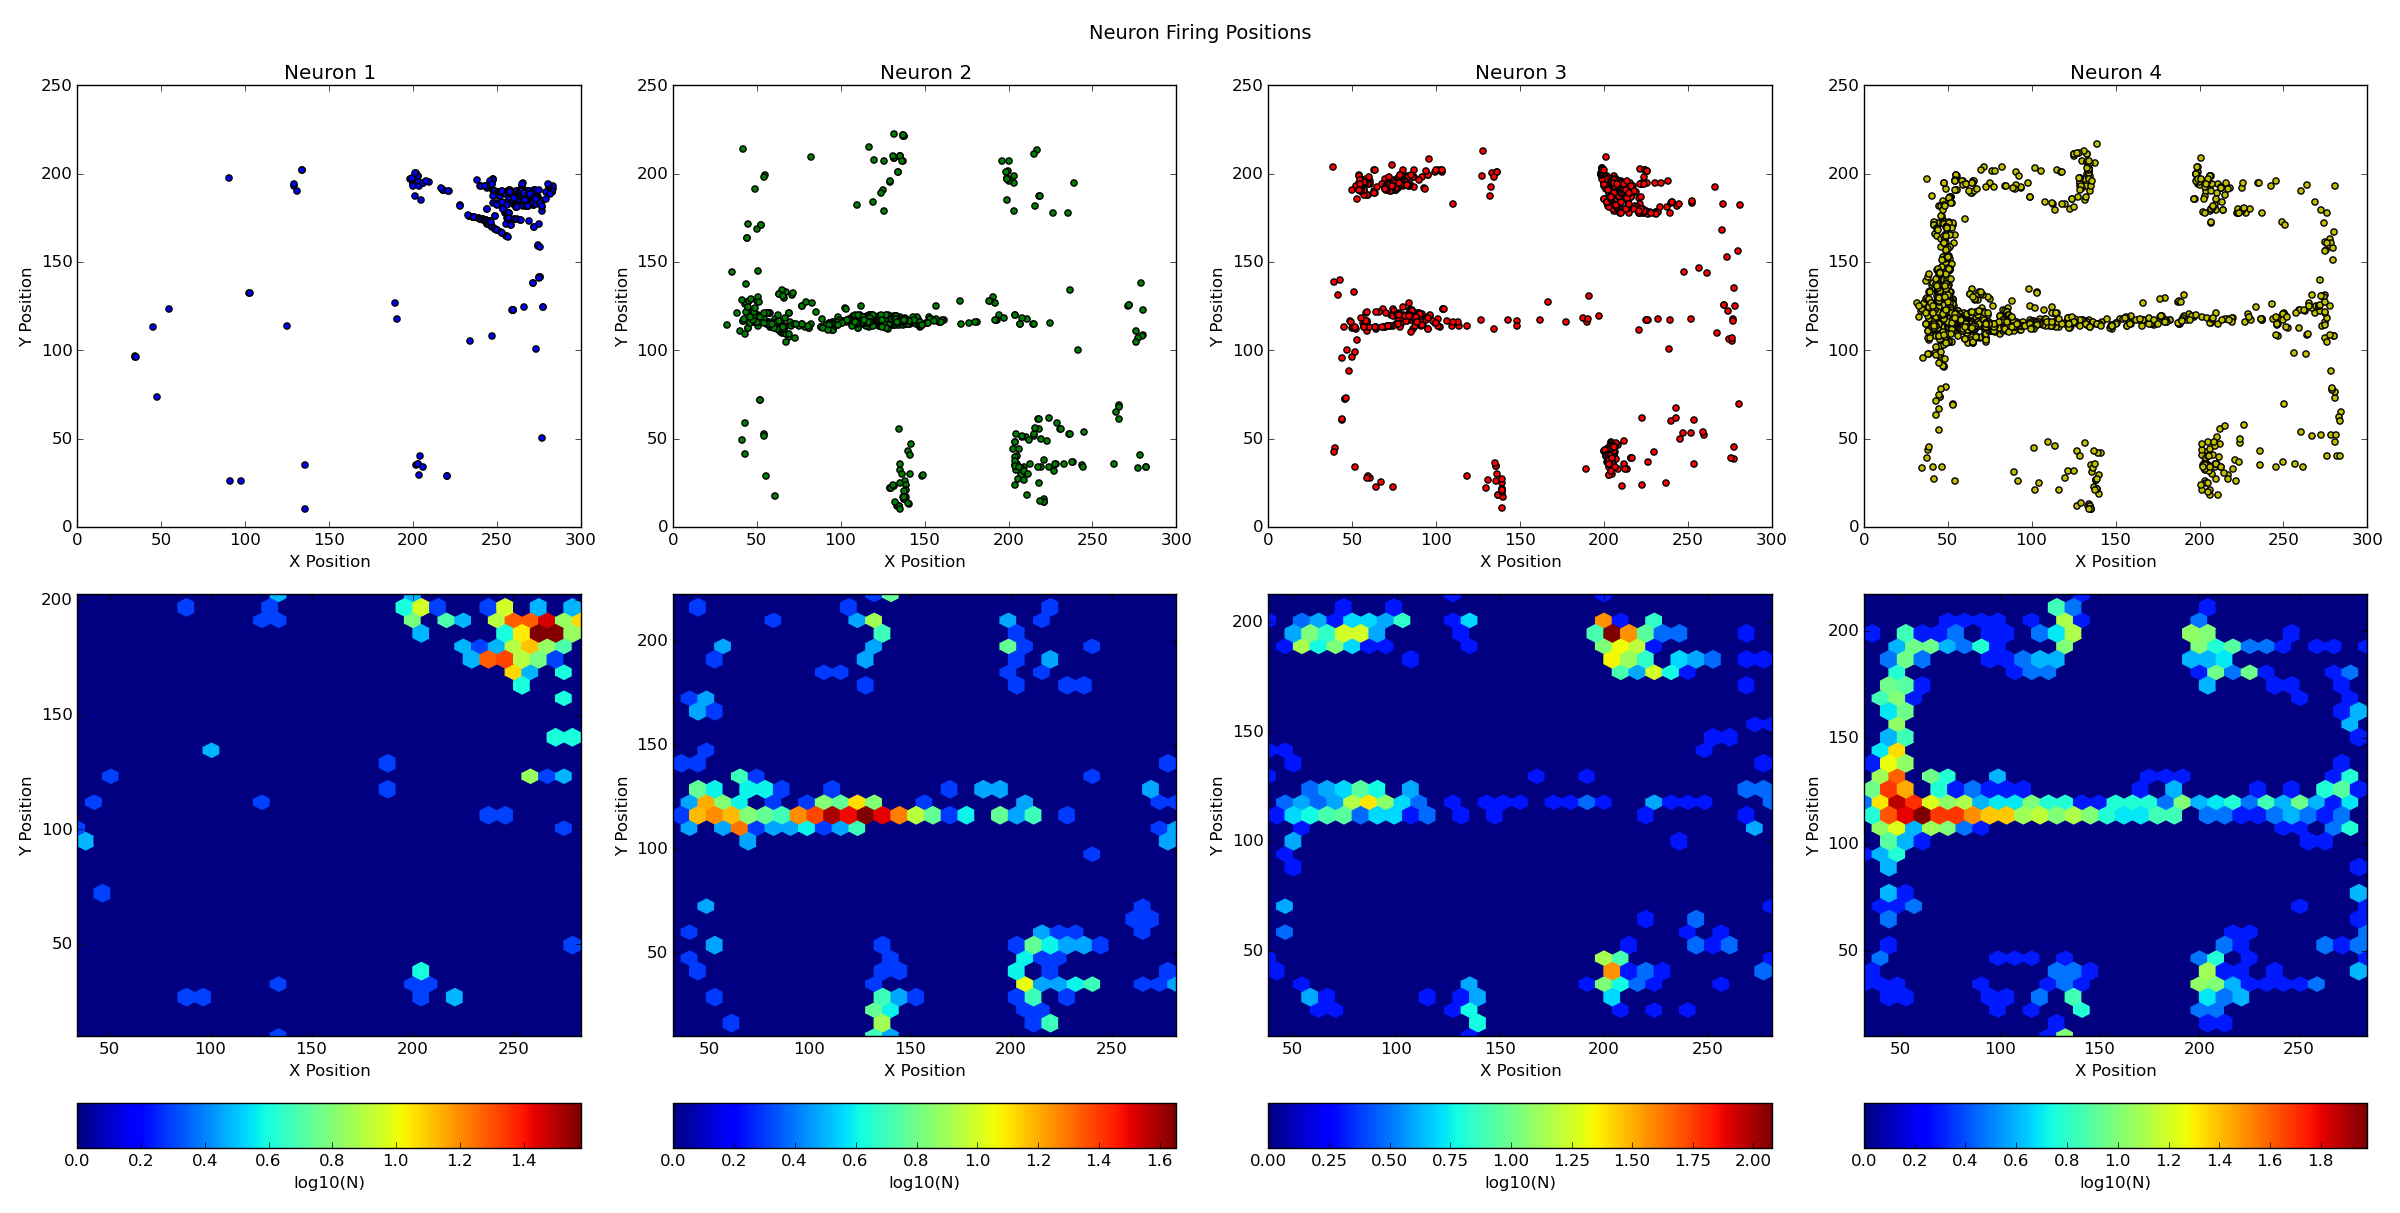
\includegraphics[width=1.0\textwidth]{neuron_pos_plot.png}
  \caption{Scatter plots and corressponding heatmaps showing the approximate location in which a spike occurred for each of the four recorded neurons.}
  \label{fig:posplot}
\end{figure}

Figure \ref{fig:posplot} shows the locations in which each neuron was most
active across multiple tests. The first neuron is active almost exclusively in
the upper right region of the maze, which suggests that this neuron is a place
cell. Place cells become active when an animal enters a corresponding place
field, but are otherwise relatively inactive. Place cells together are thought
to provide spatial processing. Neurons 2 and 4 appear to be closely
related. Neuron 2's activity is focused in the central arm of the maze. This
suggests it is involved with spatial or working memory; this neuron appears to
be involved in the recall process required to inform the choice made at the end
of the central arm. This conclusion is backed up by the activity of neuron 4,
that is most common at the end of the central arm and into the upper choice
arm. Neuron 4's apparent preference of the top arm suggests it is involved in
the decision process, using the information recalled by the second neuron. It
would be beneficial to find a corresponding neuron that showed a preference for
the opposite direction, to backup this hypothesis. Unfortunately, the function
of neuron 3 is not clear from these plots.

\subsection*{Neuron Auto-correlograms}
\begin{figure}[H]
  \centering
  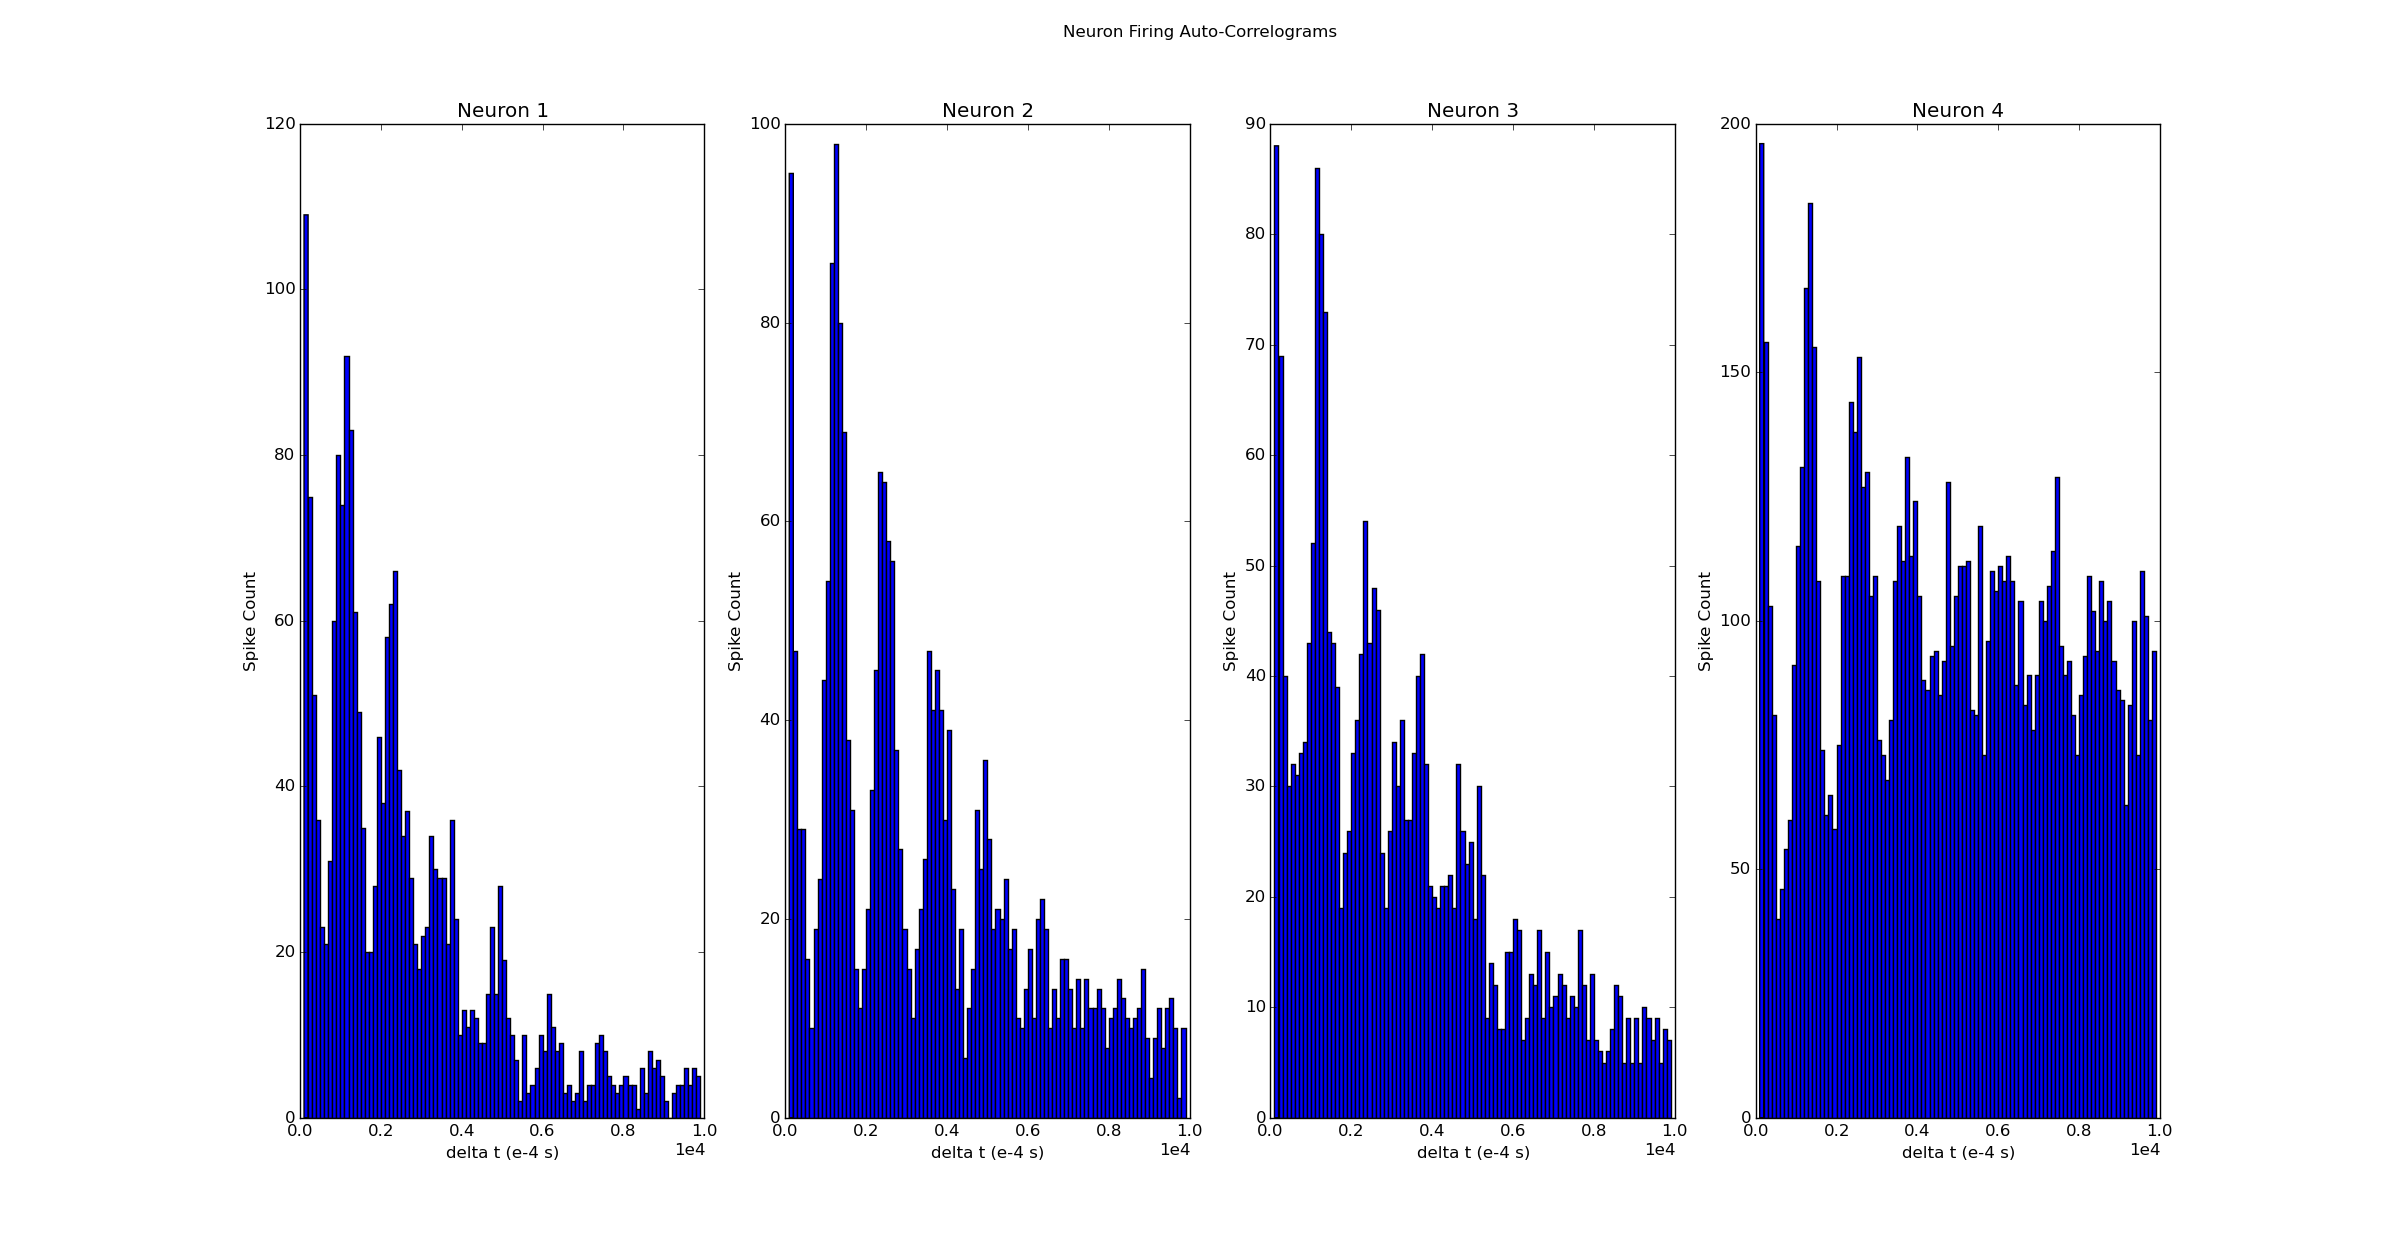
\includegraphics[width=1.0\textwidth]{neuron_acorr_plot.png}
  \caption{Auto-correlograms of neuron spike trains.}
  \label{fig:acorr}
\end{figure}

Figure \ref{fig:acorr} reveals an underlying frequency of approximately
\SI{10}{\hertz}. This shows itself as peaks representing the top half of a sine
wave with a period of roughly \SI{0.1}{\second}. This shows the presence of the
theta rhythm in the hippocampus, which is thought to be related to the
context-dependant retrieval of episodes from memory\footnote{Hasselmo, ME;
  Eichenbaum H (2005). 'Hippocampal mechanisms for the context-dependent
  retrieval of episodes'}, or as a mechanism for the relative timing of
disparate neural networks\footnote{Jones MW, Wilson MA (2005). 'Theta Rhythms
  Coordinate Hippocampal–Prefrontal Interactions in a Spatial Memory
  Task'}. Interestingly, neuron 4 exhibits a superimposed lower frequency signal
of approximately \SI{1}{\hertz}, a small portion of which is visible in the
plot.

\subsection*{Neuron Cross-correlograms}
\begin{figure}[H]
  \centering
  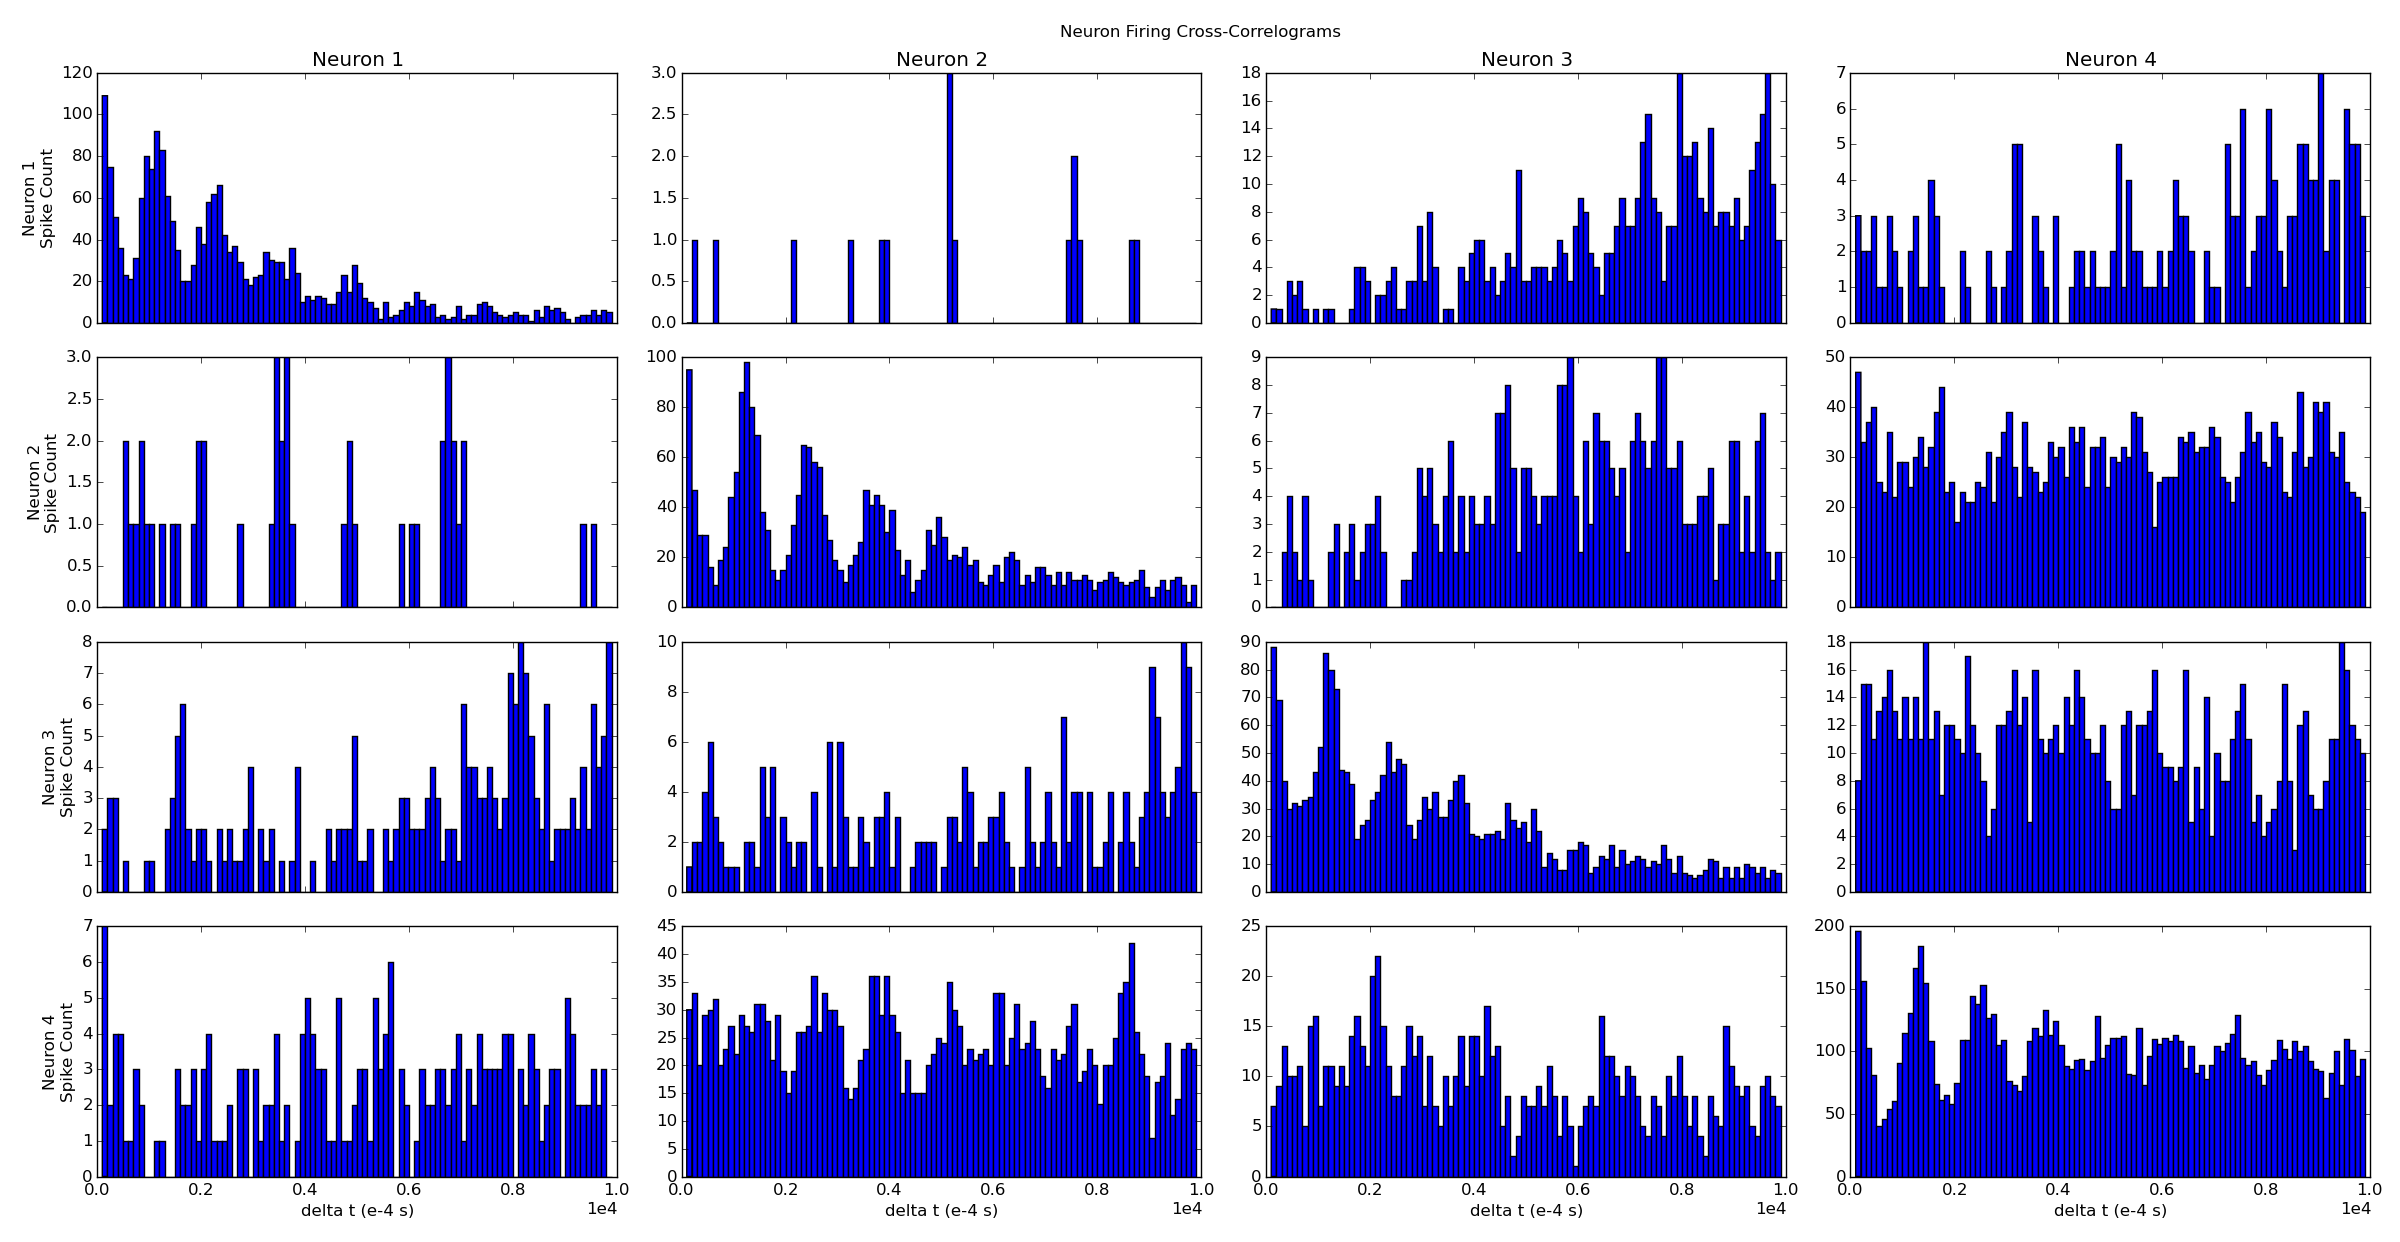
\includegraphics[width=1.0\textwidth]{neuron_xcorr_plot.png}
  \caption{Cross-correlograms of selected neuron spike train pairs.}
  \label{fig:xcorr}
\end{figure}

Figure \ref{fig:xcorr} shows some cross-correlograms of neuron
pairs. Unfortunately, the theta rhythms present in all the recorded neurons
obscure any meaningful relationships that may otherwise have been revealed
here. A quick evaluation of the two plots above shows that Neurons 2 and 4 have
little correlation, with a fairly even set of histogram heights. Neurons 1 and 3
on the other hand shows some correlation around the \SI{0.8}{\second} mark.




%% \subsection*{Part 1: Simulated Integrate and Fire Model Neuron}
%% \begin{figure}[H]
%%   \centering
%%   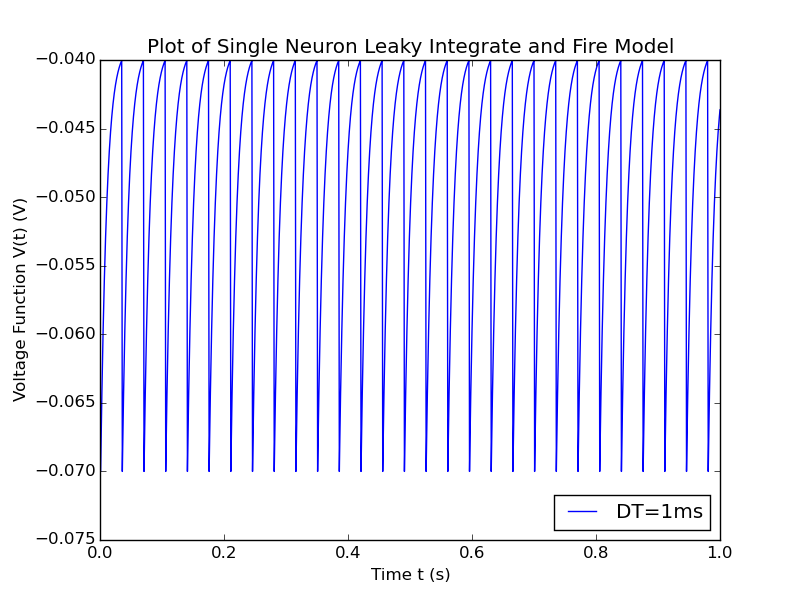
\includegraphics[scale=0.4]{p1.png}
%%   \caption{The voltage of a single neuron with fixed input current simulated with the integrate and fire model for \SI{1}{\second}.}
%%   \label{fig:n1}
%% \end{figure}

%% \subsection*{Part 2: Minimum Current for Action Potential}

%% The minimum required current, \(I_{min}\), for an action potential is \SI{3}{\nano\ampere}.

%% \begin{figure}[H]
%%   \centering
%%   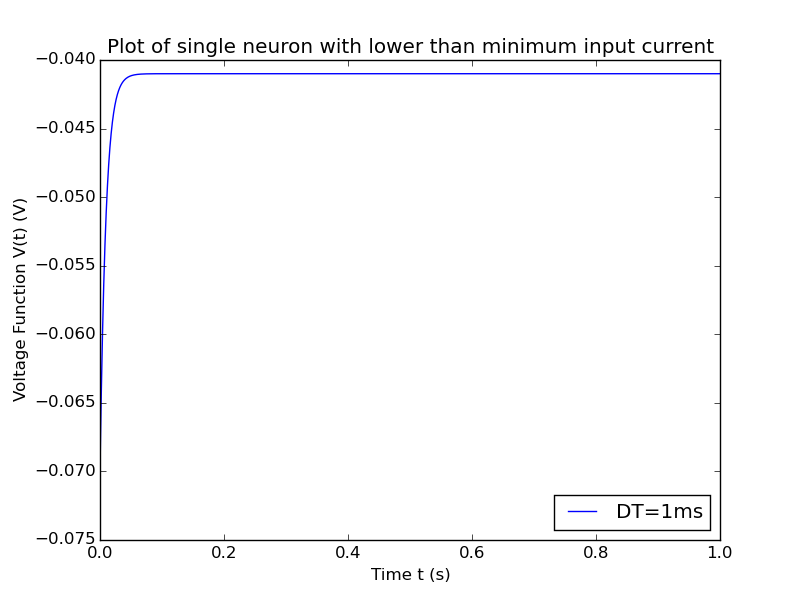
\includegraphics[scale=0.4]{p2b.png}
%%   \caption{Simulation of the neuron from Part 1 with the fixed input current reduced to \(I_{min} - \SI{0.1}{\nano\ampere}\).}
%% \end{figure}

%% \subsection*{Part 3: Simulated Firing Rate Against Input Current}

%% \begin{figure}[H]
%%   \centering
%%   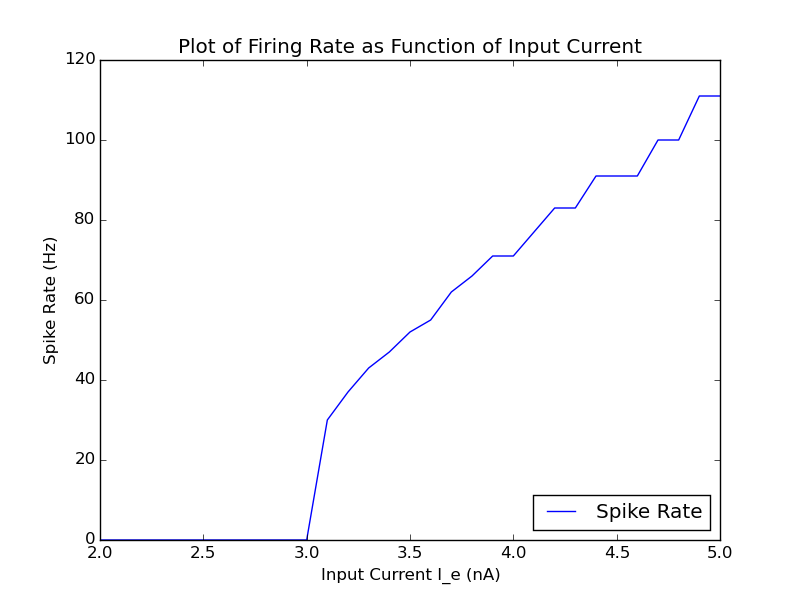
\includegraphics[scale=0.4]{p3.png}
%%   \caption{The firing rate for fixed input currents ranging from \SI{2}{\nano\ampere} and \SI{5}{\nano\ampere} sampled at \SI{0.1}{\nano\ampere} intervals, from \SI{1.0}{\second} simulations.}
%% \end{figure}

%% \subsection*{Part 4: Neuron Pair with Synaptic Connections}
%% \begin{figure}[H]
%%   \centering
%%   \begin{subfigure}{.5\textwidth}
%%     \centering
%%     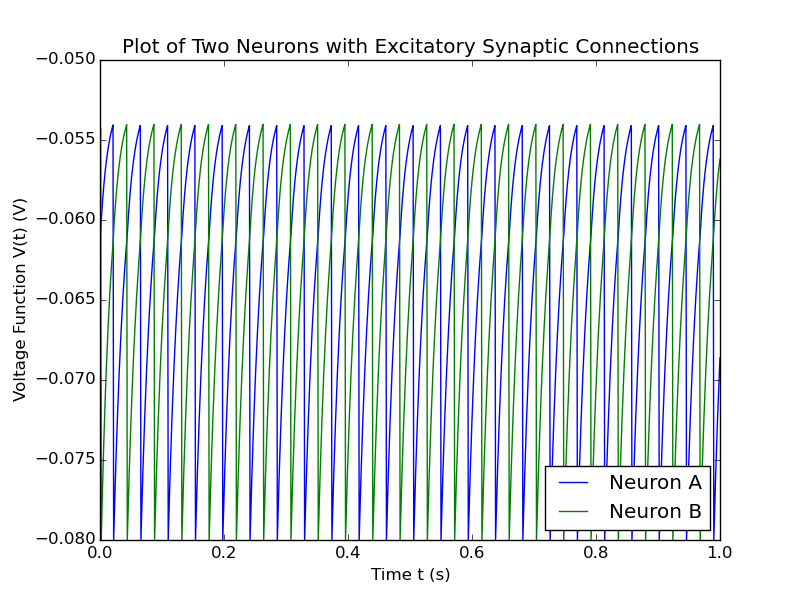
\includegraphics[scale=0.4]{p4_Excitatory.png}
%%     \caption{Excitatory Synaptic Connection}
%%     \label{fig:sub1}
%%   \end{subfigure}%
%%   \begin{subfigure}{.5\textwidth}
%%     \centering
%%     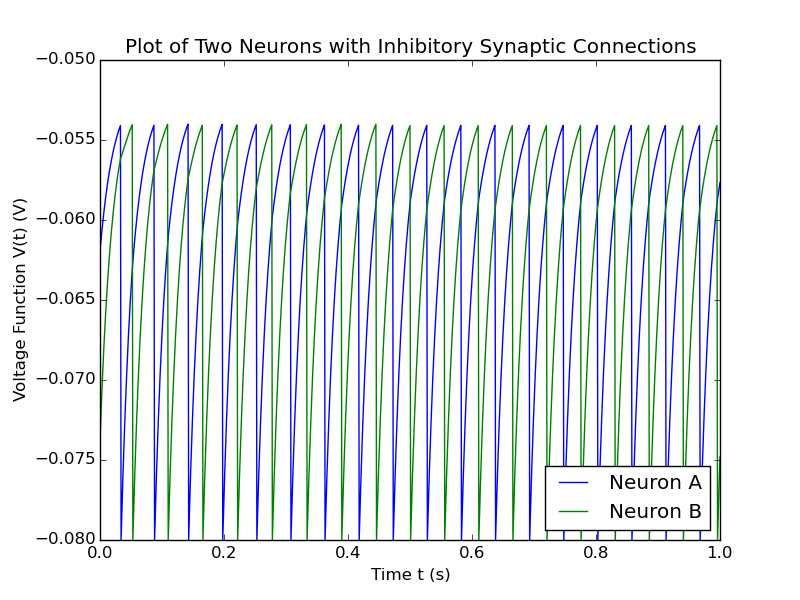
\includegraphics[scale=0.4]{p4_Inhibitory.png}
%%     \caption{Inhibitory Synaptic Connection}
%%     \label{fig:sub2}
%%   \end{subfigure}
%%   \par\medskip
%%   \caption{Plot of the voltage of two neurons with synaptic connections of differing types over time.}
%% \end{figure}

%% \vspace{5mm}
%% The excitatory synaptic connection plot in figure \ref{fig:sub1} shows that the time between spikes quickly converges. This is because when one neuron spikes, the post-synaptic neuron experiences an increase of voltage. Converseley, the inhibitory synaptic connection in figure \ref{fig:sub2} shows that the spiking frequencies become out of phase. This is due to the post-synaptic potential decreasing. In both cases, the effect is compounded as the neurons spike, causing the effect to become more pronounced (until the neurons are either completely in or out of phase, respectively.

%% \subsection*{Part 5: Slow Potassium Current}
%% \begin{figure}[H]
%%   \centering
%%   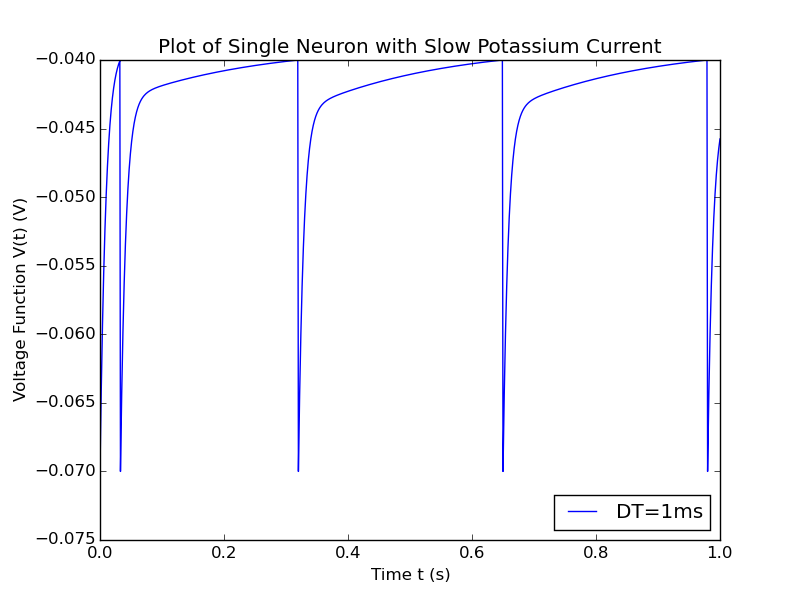
\includegraphics[scale=0.4]{p5.png}
%%   \caption{The simulated neuron shown in figure \ref{fig:n1} with an added slow potassium current.}
%% \end{figure}

\end{document}
